\documentclass[]{article}

\usepackage{graphicx}
\usepackage{pdfpages}
\usepackage{amssymb}
\usepackage{caption}
\usepackage{subcaption}
\usepackage{hyperref}
\usepackage{geometry}

%opening
\title{\vspace{-3.0cm}Insertion Sort}
\author{Yori Verbist}

\begin{document}
	
	\maketitle
	
	\section{Theoretisch vs. experiment}
	Zoals je in de onderstaande grafieken kan zien bevestigt het experiment de theorie. De theoretische lijn van de average case is een fitting van de actuele waarden zoals verwacht, dit zou dus ook bekomen worden als men het experiment meerdere keren zou runnen en het gemiddelde te nemen. \newline
	Het is ook goed te zien dat de best- en worst case gelijk zijn aan de theoretische verwachtingen. Voor de best case heb ik een array gebruikt die al reeds gesorteerd was en voor de worst case en array die van groot naar klein gesorteerd was.\newline
	Hieruit kunnen we dus ook afleiden dat bij insertion sort het veel belang heeft wat voor elementen/waarden er in de array staan en of ze al gesorteerd zijn. \newline
	 Dit verklaart ook de 'sprongen' bij de average case. Omdat deze array random waarden op random plaatsen heeft, kan het zijn dat er soms al een deel is dat grotendeels goed staat en er dus weinig vergelijkingen moeten gebeuren. Aan de andere kant kunnen er ook delen zijn die helemaal niet goed staan en daar zullen dan meer vergelijkingen moeten gebeuren. Door het experiment meerdere keren uit te voeren en het gemiddelde te nemen zullen deze 'sprongen' dus ook verdwijnen.
	
	\begin{figure}[h!]
		\centering

			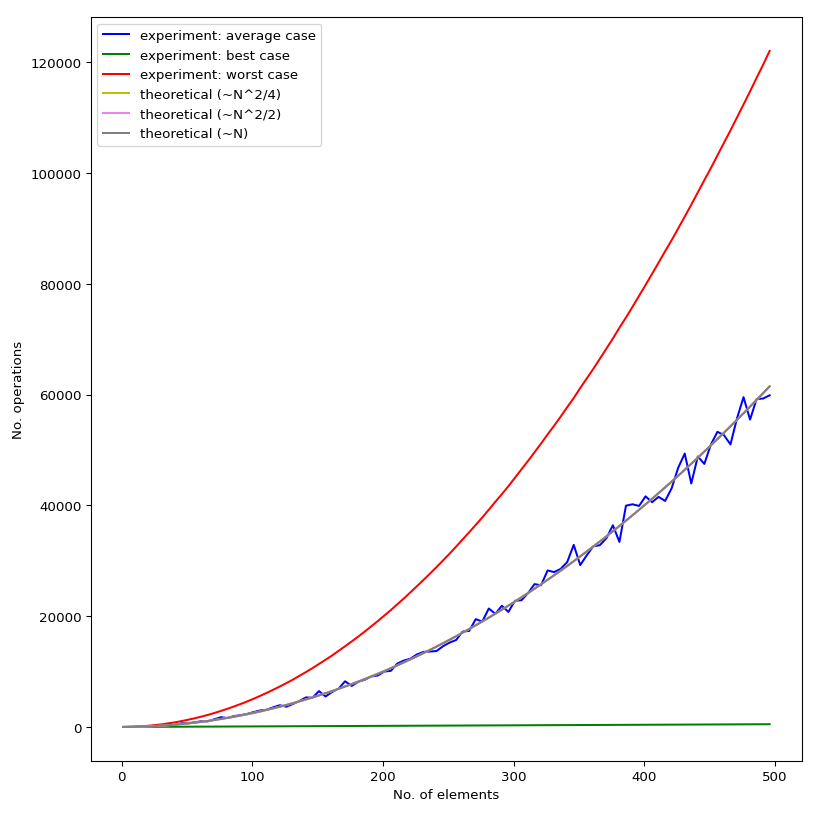
\includegraphics[width=.5\textwidth]{small}
			\caption{Lijst met 50 elementen}
	\end{figure}
	
	
\end{document}
